%% LyX 2.3.4.2 created this file.  For more info, see http://www.lyx.org/.
%% Do not edit unless you really know what you are doing.
\documentclass[12pt,english]{article}
\usepackage{ae,aecompl}
\usepackage[T1]{fontenc}
\usepackage[latin9]{inputenc}
\usepackage{geometry}
\geometry{verbose,tmargin=3cm,bmargin=3cm,lmargin=2.5cm,rmargin=2.5cm}
\usepackage{xcolor}
\usepackage{pdfcolmk}
\usepackage{float}
\usepackage{textcomp}
\usepackage{url}
\usepackage{amstext}
\usepackage{amssymb}
\usepackage{graphicx}
\usepackage{setspace}
\usepackage{esint}
\usepackage[authoryear]{natbib}
\PassOptionsToPackage{normalem}{ulem}
\usepackage{ulem}
\doublespacing

\makeatletter

%%%%%%%%%%%%%%%%%%%%%%%%%%%%%% LyX specific LaTeX commands.
\providecolor{lyxadded}{rgb}{0,0,1}
\providecolor{lyxdeleted}{rgb}{1,0,0}
%% Change tracking with ulem
\DeclareRobustCommand{\lyxadded}[3]{{\color{lyxadded}{}#3}}
\DeclareRobustCommand{\lyxdeleted}[3]{{\color{lyxdeleted}\lyxsout{#3}}}
\DeclareRobustCommand{\lyxsout}[1]{\ifx\\#1\else\sout{#1}\fi}

%%%%%%%%%%%%%%%%%%%%%%%%%%%%%% User specified LaTeX commands.
%\usepackage{aecompl}
\usepackage{ae,lmodern}
\usepackage{lineno}

\usepackage{babel}

%\linenumbers
\date{}

\makeatother

\usepackage{babel}
\begin{document}
\title{Looking for compensation at multiple scales in a wetland bird community}
\author{{\Large{}{}Fr?d?ric Barraquand$^{1,2,*}$, Coralie Picoche$^{1,2}$,
Christelle Aluome$^{1,3}$, }\\
 {\Large{}{}Laure Carassou$^{1,4}$ \& Claude Feign?$^{5}$}}

\maketitle
{\large{}{}\bigskip{}
}{\large\par}

{\large{}{}}\textsuperscript{{\large{}{}1}}{\large{}{}~University
of Bordeaux, Integrative and Theoretical Ecology, LabEx COTE, B?t.
B2 - All?e Geoffroy St-Hilaire, 33615 Pessac, France \bigskip{}
}{\large\par}

{\large{}{}}\textsuperscript{{\large{}{}2}}{\large{}{}~CNRS, Institute
of Mathematics of Bordeaux, 351 Cours de la Lib?ration, 33405 Talence,
France}{\large\par}

{\large{}{}\bigskip{}
}{\large\par}

{\large{}{}}\textsuperscript{{\large{}{}3}}{\large{}{}~ISPA, Bordeaux
Sciences Agro, INRA, 33140 Villenave d'Ornon, France}{\large\par}

{\large{}{}\bigskip{}
}{\large\par}

{\large{}{}}\textsuperscript{{\large{}{}4}}{\large{}{}~INRAE,
UR EABX, 50 Avenue de Verdun, 33612 Cestas, France}{\large\par}

{\large{}{}\bigskip{}
}{\large\par}

{\large{}{}}\textsuperscript{{\large{}{}5}}{\large{}{}~PNR Landes
Gascognes, Teich Ornithological Reserve, Rue du Port BP 11 33470 Le
Teich, France}{\large\par}

{\large{}{}\bigskip{}
}{\large\par}

{*} Corresponding author. Email: frederic.barraquand@u-bordeaux.fr

\thispagestyle{empty}

\pagebreak{}

%\linenumbers

\begin{linenumbers}{
\begin{abstract}
Compensatory dynamics, during which community composition shifts despite
a near-constant total community size, are usually rare: synchronous
dynamics prevail in natural communities. This is a puzzle for ecologists,
because of the key role of compensation in explaining the relation
between biodiversity and ecosystem functioning. However, most studies
so far have considered compensation in either plants or planktonic
organisms, so that evidence for the generality of such synchrony is
limited. Here, we extend analyses of community-level synchrony to
wetland birds. We analyse a 35-year monthly survey of a community
where we suspected that compensation might occur due to changes in
water levels, favouring birds with different habitat preferences,
and potential competition. We perform both year-to-year analyses by
season, using a compensation/synchrony index, as well as multiscale
analyses using a wavelet-based measure, which allows for both scale-
and time-dependence. We analyse synchrony both within and between
guilds, with guilds defined either as tightknit phylogenetic groups
or larger functional groups. We find that abundance and biomass compensation
is rare, likely due to the synchronizing influence of climate (and
other drivers) on birds, even after considering several temporal scales
of covariation (during either cold or warm seasons, above or below
the annual scale). Negative covariation in abundance at the guild
or community level did only appear at the scale of a few months or
several years. We also found that synchrony varies with taxonomic
and functional scale: the rare cases where compensation appeared consistently
in year-to-year analyses were \emph{between} rather than \emph{within}
guilds, using functional groups. Our results suggest that abundance
compensation may have more potential to emerge between broad functional
groups rather than between species, as well as at relatively long
temporal scales (multiple years for vertebrates), above that of the
dominant synchronizing driver.
\end{abstract}
\textbf{Keywords: }compensation; synchrony; biodiversity; birds; time
series; wavelets

\newpage{}

\section*{Introduction}

Density compensation occurs when individuals of a given species replace
individuals of other species within a community, either because of
explicit competitive processes or shifts in environmental drivers
that change selection pressures \citep{gonzalez2009causes}. The community
as a whole then exhibits lower abundance variation than its constituent
species \citep{gross2013species}: some degree of compensation or
asynchrony is therefore a prerequisite to stabilization at the community
level \citep{loreau2013biodiversity}.

Understanding why environmental variation may lead to compensation
is relatively easy: if species have different environmental preferences
(e.g., thermal optima), and the environment changes over time, different
species will be fittest at different points in time. As a consequence,
relative abundances will shift over time even though the community
abundance or biomass as a whole may remain relatively stable \citep{gonzalez2009causes}.
However, the conditions for compensation to happen also depend on
the particulars of the interactions between and within species in
the community.

Compensation is particularly likely to occur when temporal environmental
variation combines with a space constraint or with a strongly limiting
resource, so that individuals are close to competing in a zero-sum
game (sensu \citealp{hubbell2001unified} or lottery-style models,
\citealp{chesson_multispecies_1994}). When the total community size
is constant over time, and the composition fluctuates, negative covariation
between abundances then emerges by design \citep{loreau_species_2008}
since no species can increase without at least another species decreasing
in abundance. Outside of this zero-sum scenario, in models where Lotka-Volterra
competition is combined with temporal environmental variability, theoretical
research has revealed that increased interspecific competition might
not always increase species compensation \citep{ives_stability_1999}
and might even decrease it \citep[i.e., increase species synchrony instead,][]{loreau_species_2008,loreau2013biodiversity},
though this depends on the fluctuation regime. Thus, in a world where
total community size varies, predicting whether compensatory dynamics
can occur is intrinsically difficult \citep{klink_functional_2019}.

Early investigations of the frequency of synchronous vs compensatory
dynamics focused on the variance ratio, that is, the variance of the
sum of the community biomass divided by the sum of the variance of
the component species biomasses \citep{houlahan_compensatory_2007,gonzalez2009causes}.
Unfortunately, this metric is not appropriate for communities subjected
to community-wide environmental forcing \citep{ranta_detecting_2008},
because a main environmental driver (e.g., temperature or light) may
synchronize species abundances or growth rates at some temporal scale,
creating large variance in community-wide biomass, in spite of strongly
competitive dynamics. Further research has therefore focused on specific
timeframes during which compensatory dynamics may be found (e.g.,
below the annual scale at which temperature fluctuations tend to synchronize
species dynamics, \citealp{vasseur_synchronous_2014}).

Despite efforts to look for more meaningful temporal scales in community-level
time series, temporal compensation has remained surprinsingly elusive
in the field \citep{houlahan_compensatory_2007,vasseur_synchronous_2014};
but see \citet{ernest2008zero,christensen2018long}. Most datasets
used so far to evaluate temporal compensation vs synchrony involve
planktonic organisms \citep{vasseur2007spectral,vasseur_synchronous_2014}
or terrestrial plants (\citealp{bai2004ecosystem,houlahan_compensatory_2007,gross2013species};
though see \citealp{bell_stability_2014} in fishes, \citealp{ernest2008zero}
in mammals and \citealp{klink_functional_2019} in beetles). Here,
we take advantage of a long-term bird abundance time series in a natural
reserve, with records every month for 35 years, allowing us to dig
deeper into patterns of synchrony, at several temporal and taxonomic
or functional scales.

Taxonomic and functional scales should indeed be main modulators of
synchrony/compensation. On the one hand, compensation can be high
between similar and closely related species. If two species of ducks
A and B share almost the same niche, individuals from either species
experience similar competition from species A or B, and should feel
the effects of other species in the community identically. This favours
priority effects \citep{fukami_historical_2015}, with chance due
to movement events determining whether species A or B locally dominates,
which can then provide compensation at the landscape level \citep{loreau2003biodiversity}.
On the other hand, it could be argued that these two similar duck
species will precisely respond in similar ways to environmental variables,
which tends to obfuscate compensation. Hence, more dissimilar species
or groups (within the same trophic level nonetheless) could exhibit
more compensation \citep{bai2004ecosystem,morin2014temporal,klink_functional_2019}
because they are more likely to respond to the environment in an asynchronous
manner (\emph{sensu} \citealp{loreau2013biodiversity}). Surprisingly,
such compensation \textit{between} guilds has been less well explored
empirically than \emph{within} guilds, even though there is actually
some empirical evidence for compensation between dissimilar guilds
\citep[e.g.,][]{bai2004ecosystem,roscher_identifying_2011,sinclair2013asynchronous,klink_functional_2019}.
In this paper, we explore the level of compensation/synchrony within
or between guilds of a wetland bird community, along either taxonomic
or functional classifications. Although a functional classification
might appear intuitively more appealing, our knowledge of functional
traits is necessarily partial and imperfect, so that a taxonomic description
can sometimes be preferable \citep{clark_why_2016}. Our dataset is
ideally suited to examine the presence of synchrony or compensation
at different scales given that (i) it is a highly temporally resolved
time series with respect to the species typical generation times,
but it also extends well beyond generation time (timespan of 35 years)
and (ii) the reserve where the data has been collected was subjected
to a major management change c. 2006 (change in water levels), favouring
different types of wetland birds (so that over long timescales, there
is a real potential for changes in community composition).

\section*{Material and Methods}

\subsection*{Data}

The monthly time series used for the statistical analyses have been
collected at the Teich Ornithological Reserve, Arcachon Bay, France
(44.64?N / -1.02?E), by the staff of the Teich reserve, over the whole
study period (1981-2016). A species list of the frequent birds is
provided in SI Appendix S1. The reserve comprises 120 ha of wetlands,
and the counts have been aggregated at the reserve scale (summed over
18 sectors where the counts are actually performed, using binoculars).
We use for each species the maximum observed abundance over a month,
which provides a ``monthly snapshot'' of the bird abundance, that
has been used to monitor the reserve since its inception. When abundance
values are not reported for certain species and months, we replace
them by zeroes. Given the sustained observation effort (all sectors
are patrolled multiple times throughout the month by the staff, amateur
ornithologists visiting the reserve daily and communicating their
findings to the reserve staff), we consider that the absence of counts
for a given species signals its true absence from the reserve. This
creates some zero abundances for rare species at the monthly scale.
We have not attempted to ``correct'' those zeroes (e.g., inferring
the ``missing'' data with a model assuming that our reserve is a
subsample of a regional population) because doing so would have compromised
the patterns of local synchrony/compensation. However, we did check
that having such zeroes in the monthly time series cannot affect our
conclusions (see SI). In the statistical analyses, we use seasonally
averaged abundances (plotted in Fig. \ref{fig:Temporal-trends}),
as well as the original monthly data (presented in Appendix S2). We
defined two seasons based on observations of bird presence. We defined
a `warm season', from May to August, and a `cold season' as the months
between November and February of the following year. From an ecological
viewpoint, this seasonal classification separates wintering birds
from summer residents (some of whom are breeding). This makes sense
biologically because the two communities have different requirements
and could respond differentially to abiotic drivers. It is also useful
from a more statistical perspective, as there is a partial shift in
composition between the seasons, though winter and summer communities
greatly overlap (i.e., species with greater abundances in the reserve
in winter have also some summer residents, though these may be different
individuals). The dynamics of species abundances in the Teich reserve
bird community show a marked signature of seasonality (Fig. \ref{fig:Temporal-trends}).

\begin{figure}[H]
\begin{centering}
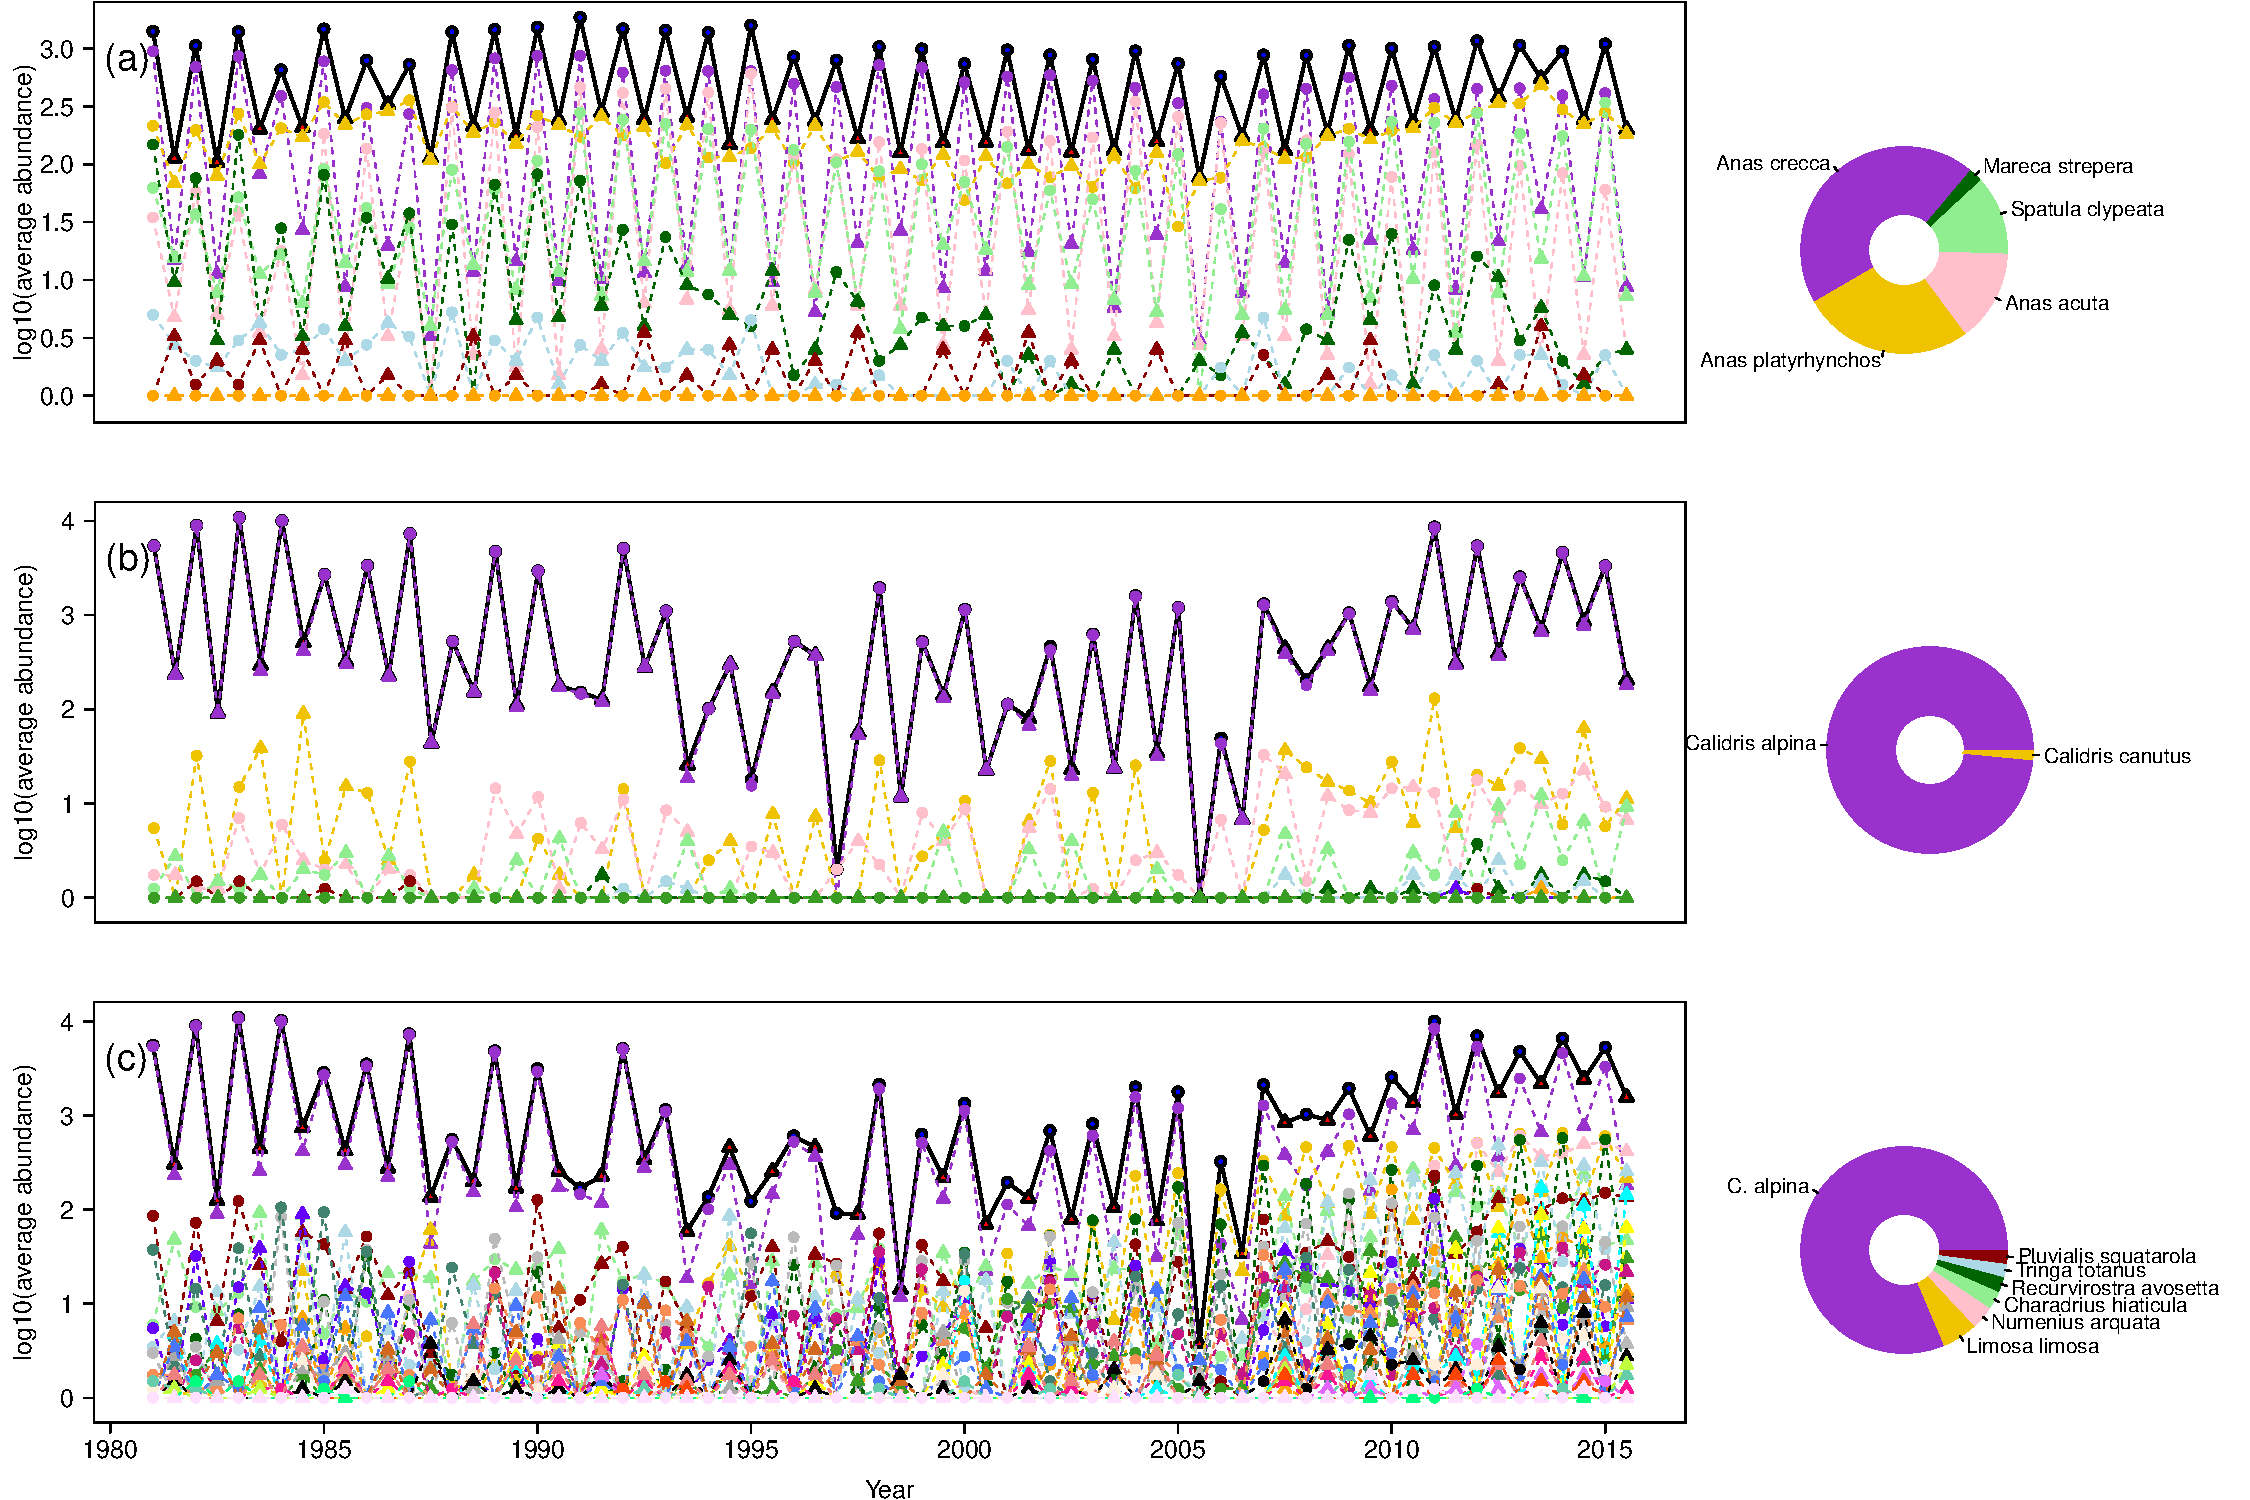
\includegraphics[width=18cm]{average_abundance_timeseries_v2}
\par\end{centering}
\caption{Time series of seasonally averaged abundance for\emph{ }ducks of the
tribe\emph{ Anatini} (a), calidrids (b, \emph{Calidris} genus), and
all waders (c, including calidrids). The solid black lines (on top
of each panel) represent the summed average abundances for each guild,
dotted lines represent average abundance for each species. Circles
represent the cold season and triangles, the warm season. The coloured
symbols below the curves represent each species abundances, with
species composition on the right side on the donut plots for the most
abundant species (over 1\% of relative abundance in the group considered).
We added 1 to abundances before log-transforming to avoid issues with
zero values. \label{fig:Temporal-trends}}
\end{figure}


\subsection*{Bird taxonomic and functional groups}

The reserve is dominated by waders and waterfowl (ducks, geese and
swans). These two functional groups collectively represent 68\% of
the total number of observed birds over the years and are always present
on site. Two fairly common phylogenetic groups, both in abundance
and occurrence, are members of the \emph{Anatini }tribe (corresponding
previously to the \emph{Anas} genus, \citealp{gonzalez_phylogenetic_2009})
in ducks and members of the \emph{Calidris} genus in waders. Waders
and ducks have different environmental preferences, with ducks (and
waterfowl more generally) preferring water levels allowing them to
dabble (or dive for \emph{Aythini}), while waders usually forage on
mudflats. A list of all birds found frequently in the reserve is presented
in Appendix S1; aside from waders and waterfowl, other common species
include herons, egrets and cormorants (see below). Among the fish
eaters, grebes and gulls were frequently counted; a few raptors were
present as well.

To examine compensation \emph{between} and \emph{within} the waders
and waterfowl categories, we contrasted analyses using a taxonomic
classification of the species (i.e., between and within phylogenetic
groups such as genera) and a functional classification of the species
(26 species of waders vs 17 species of waterfowl). The waterfowl group
includes all anatids (ducks, geese and swans in particular) as well
as the common coot \emph{(Fulica atra}, an abundant species here,
which is a Rallidae but resembles a duck in morphology and foraging
habits; hence its inclusion).

In addition to our main analyses on waders and waterfowl, we also
``zoomed in'' on a set of species that were known to exhibit potentially
compensatory dynamics through competition for roosting sites: the
great cormorant \textit{(Phalacrocorax carbo)}, the little egret (\textit{Egretta
garzetta}) and the grey heron (\textit{Ardea cinerea}). The little
egret and grey heron abundances were summed because of their similar
requirements (i.e., they form a small functional group).

\subsection*{Statistical Analyses}

\subsubsection*{Year-to-year analyses}

We used for year-to-year analyses the synchrony index $\eta$ defined
by \citet{gross2013species}, which is constructed as the mean cross-correlation
between each species abundance and the summed abundances of the rest
of the community (eq. \ref{eq:Gross}):

\begin{equation}
\text{\ensuremath{\eta}}=\frac{1}{n}\sum_{i}\text{Corr}(X_{i},\sum_{j\neq i}X_{j})\label{eq:Gross}
\end{equation}

where $X_{i}$ is the abundance or biomass of species $i$ in a community
of $n$ species and the correlation is computed over the years. This
synchrony index varies between -1 (perfect compensation, total abundance
is constant) and 1 (complete synchrony), while 0 represents a case
where populations fluctuate independently on average. Contrary to
other indices (e.g., \citet{loreau_species_2008}'s $\phi$), this
index is independent from the richness $n$ of the community (or more
generally the number of system components) and its overall stability
\citep{bluthgen_land_2016,hallett_codyn_2016}. This is particularly
important here as we perform analyses at different taxonomic scales,
and therefore with a different $n$ in eq. \ref{eq:Gross}. All analyses
performed with abundance in the main text are performed with biomass
in Supporting Information Appendix S4.

We computed the synchrony index $\eta$ over all available years,
but separately for cold and warm seasons, using the \verb|codyn|
package in R \citep{hallett_codyn_2016}. That is, we constructed
two community-level time series of species abundances, one for the
cold season and one for the warm season. To do so, we averaged monthly
bird abundances, for each species, over the season duration. In follow-up
analyses, we also differentiated periods before and after 2006, given
that a management change occurred within the reserve in 2006. We considered
both the synchrony within a given guild (e.g., among species of the
\textit{Calidris} genus) or between guilds (e.g., between the summed
abundances of the 7 species of tribe \textit{Anatini} and\emph{ }\textit{\emph{the
sum of the 6 }}\textit{Calidris} species). In the latter case of between-guilds
comparisons, we summed species together before seasonal averaging,
to consider seasonal averages of the monthly guild-level abundance.
Finally, we computed $\eta$ within the community of the 60 most frequent
birds.

We computed the statistical significance of the synchrony index by
comparing the observed values to the distribution of $\eta$ under
the null hypothesis \citep{gouhier_synchrony_2014}, which amounts
to cross-correlations of value zero between species abundances (or
guild-level abundances, when considering taxonomic or functional groups).
The challenge, in order to construct such null hypothesis, is to remove
all cross-correlations while keeping the exact same autocorrelation
in each individual time series. Therefore, for each set of time series
(each combination year $\times$ season for a given community), we
constructed 1000 ``surrogates'' in which we kept auto-correlations
but removed cross-correlations between time series. There are multiple
ways to erase cross-correlations depending on the resolution of the
considered community. Within guilds, we shifted the time-series \citep{purves_fine-scale_2002}
while between guilds (two groups only), we used a frequency-based
approach (Iterative Amplitude-Adjusted Fourier Transform or IAAFT,
see \citealp{schreiber_surrogate_2000}). We first explain the shift-based
approach: the suite of abundance values (after seasonal averaging)
is displaced by a random temporal lag $\tau$, so that a value $y_{t}$
is now found at $y_{t+\tau}$. At the boundary (the end of the time
series), remaining points are displaced towards the beginning of the
time-series, which implements a toroidal shift. This method works
well when comparing many times series corresponding to the multiple
species. However, when computing synchrony across only two groups
(between guilds), spurious cross-correlations could emerge with a
shift-based approach as the number of possible combinations is more
limited. Therefore, to test for synchrony between the summed abundances
of two guilds or taxonomic units, we used the more sophisticated IAAFT
method \citep{schreiber_surrogate_2000}, which retains the frequency
spectrum of the time series while randomising its values. We obtained
1000 sets of randomised time series for each computed synchrony index.
We then compared the number of $\eta_{H0}$ values which exceeded
or were inferior to the observed value to compute the p-value \citep{north_note_2002}:
we use the ratio $(r+1)/(n+1)$ where $r$ is the number of surrogate
values that are $\ge\eta_{obs}$ or $\le\eta_{obs}$, and $n$ is
the number of surrogates. Independence of species was rejected at
the 10\% threshold with a Benjamini-Hochberg correction, as we compare
across 2 seasons and 3 periods (all years, before 2006, after 2006),
with partially overlapping data. This was found satisfactory based
on simulated data, although power is low for detecting compensation
(i.e., the null cannot always be rejected) when only two groups are
compared.

\subsubsection*{Wavelet analyses}

In addition to the time-domain analyses above, we performed wavelet
analyses at multiple temporal scales, ranging from a month to several
years. Wavelet analyses provide information on community synchrony
for a given temporal scale or frequency, as well as a given location
in time along the time series. This was done at the whole community
level, including the 60 most frequent bird species, and for the rich
wader and waterfowl communities, as well as the group formed by the
great cormorant, grey heron and little egret. All wavelet analyses
take as input the monthly time series data. Based on the work by \citet{keitt_coherent_2008}
and follow-up by \citet{vasseur_synchronous_2014}, we used the wavelet
modulus ratio to measure the synchrony between time series

\begin{equation}
\rho(t,s)=\frac{\int_{-\infty}^{+\infty}\frac{1}{\sqrt{2\pi}}e^{-\frac{1}{2}(\frac{\tau-t}{s})^{2}}|\sum_{i}w_{i}(\tau,s)|d\tau}{\int_{-\infty}^{+\infty}\frac{1}{\sqrt{2\pi}}e^{-\frac{1}{2}(\frac{\tau-t}{s})^{2}}\sum_{i}|w_{i}(\tau,s)|d\tau}\label{eq:Keitt}
\end{equation}

where $w_{i}(t,s)$ is the continuous Morlet wavelet transform of
species $i$ at time $t$ for scale $s$, and $|\centerdot|$ is the
modulus of the complex number. The numerator considers the total abundance
variation $|\sum_{i}w_{i}(\tau,s)|$ at a given temporal scale $s$
and location in time $\tau$, while the denominator considers a weighted
sum of the fluctuation amplitude of each species ($\sum_{i}|w_{i}(\tau,s)|$).
The Gaussian weights in the numerator and denominator ensure that
$\rho(s,t)$ is specific to scale $s$ and time $t$. This index $\rho$
is close to 0 when species (or compartments) compensate and reaches
1 when they are synchronous \citep{keitt_coherent_2008}. Significance
of high and low values of $\rho$ were evaluated using a 10\% overall
level. The null hypothesis was constructed using the IAAFT algorithm
\citep{schreiber_surrogate_2000}, using 1000 surrogate time series,
and computing of the corresponding $\rho$ values for each one \citep[similar to][]{cazelles2014wavelet}.
The robustness of the wavelet approach to the presence of exactly
zero values is tested in SI Appendix S6. Appendices S7 and S8 further
test the ability of $\rho$ to identify compensation or synchrony
in cases of skewed species abundance distribution, either in the mean
or in the amplitude of temporal variation.

Statistical significance testing was always done using a significance
level $\alpha$ = 10\%, which was based on previous experience working
with (statistically short) ecological time series as well as analyses
of numerical simulations using $\alpha$ = 10\%, provided in SI Appendices.

All datasets and statistical analyses are available in a GitHub repository
\url{https://github.com/fbarraquand/BirdTimeSeries_Teich} and stored
at Zenodo {[}will be done for the final version{]} (Picoche, Aluome
\& Barraquand, 2020). Finally, we want to highlight a conceptual issue
worth keeping in mind: both $\rho$ and $\eta$ indicate synchrony
when reaching one, but such synchrony should be understood as the
reciprocal of compensation rather than exactly synchronized peaks
and troughs for all species (i.e., phase synchrony). Unlike phase
synchrony, compensation and community-level synchrony depend on the
distribution of abundance variation within the community. In the limit
case where a single species abundance fluctuates more than all others
combined, compensation may not even be reachable, since variation
in the abundance of that dominant species cannot be offset by changes
in numbers of other species. Only when species densities have commensurate
temporal variability will the concepts of community-level synchrony
and phase synchrony exactly match.

\section*{Results}

\subsection*{Synchrony within phylogenetic or functional groups}

Using a taxonomic classification of the community, \textit{\emph{focusing
on the genera}} \textit{Calidris} and tribe \textit{Anatini }\textit{\emph{(formerly
}}\textit{Anas}\textit{\emph{)}} as two key examples of taxonomic
units with contrasted preferences, within-genus synchrony dominates
year-to-year analyses for the two seasons (Fig. \ref{fig:Gross-synchrony-index}).
Using functional groups (waders and waterfowl), synchrony within functional
groups was also prominent. The \citet{gross2013species} synchrony
indices are indeed mostly positive, and always positive whenever significantly
different from the null hypothesis of no temporal correlation between
species. Therefore, there is no compensation within guilds (Fig. \ref{fig:Gross-synchrony-index}a
and b) across years, for the two seasons. This matches the patterns
obtained within the entire wetland bird community (Fig. \ref{fig:synchrony-whole-comm}a):
synchrony dominates when abundances are computed at the species level.

For the cold season, abundances within \textit{Calidris} and \textit{Anatini}
display opposite changes in synchrony values in response to the management
change in 2006, with species within \emph{Anatini} becoming less synchronous
over time, although we should mention that these changes are not statistically
significant. For the warm season, the management change, which consisted
of lowering the water levels, created little change in communities
of species within the \emph{Anatini} and \emph{Calidris}: they are
all synchronous.

Even though there is no widespread community-wide or genus-wide compensation
across years (separating the two seasons), there could be compensation
at finer temporal scales, e.g. a month or two, or coarser scales,
over several years. Such compensation could also occur at specific
time intervals instead of throughout the whole time series, a time-dependency
that wavelet analyses allow to reveal. When we consider the wavelet
modulus ratio (Fig. \ref{fig:Wavelet-modulus-ratio}), that is, a
time-varying and scale-dependent strength of synchrony, we can see
that there is synchrony even at a fine temporal scale throughout most
of the time series. However, post-2006, there seems to be a possibility
for episodic compensation on a temporal scale of approximately 2-4
months, for both waders and waterfowl. There could also be within-guild
compensation at scales of 5 years, approximately post-2000 for waders
and pre-2005 for waterfowl. Waterfowl synchrony trends likely influence
whole-community trends (Fig. \ref{fig:synchrony-whole-comm}).

\begin{figure}[H]
\begin{centering}
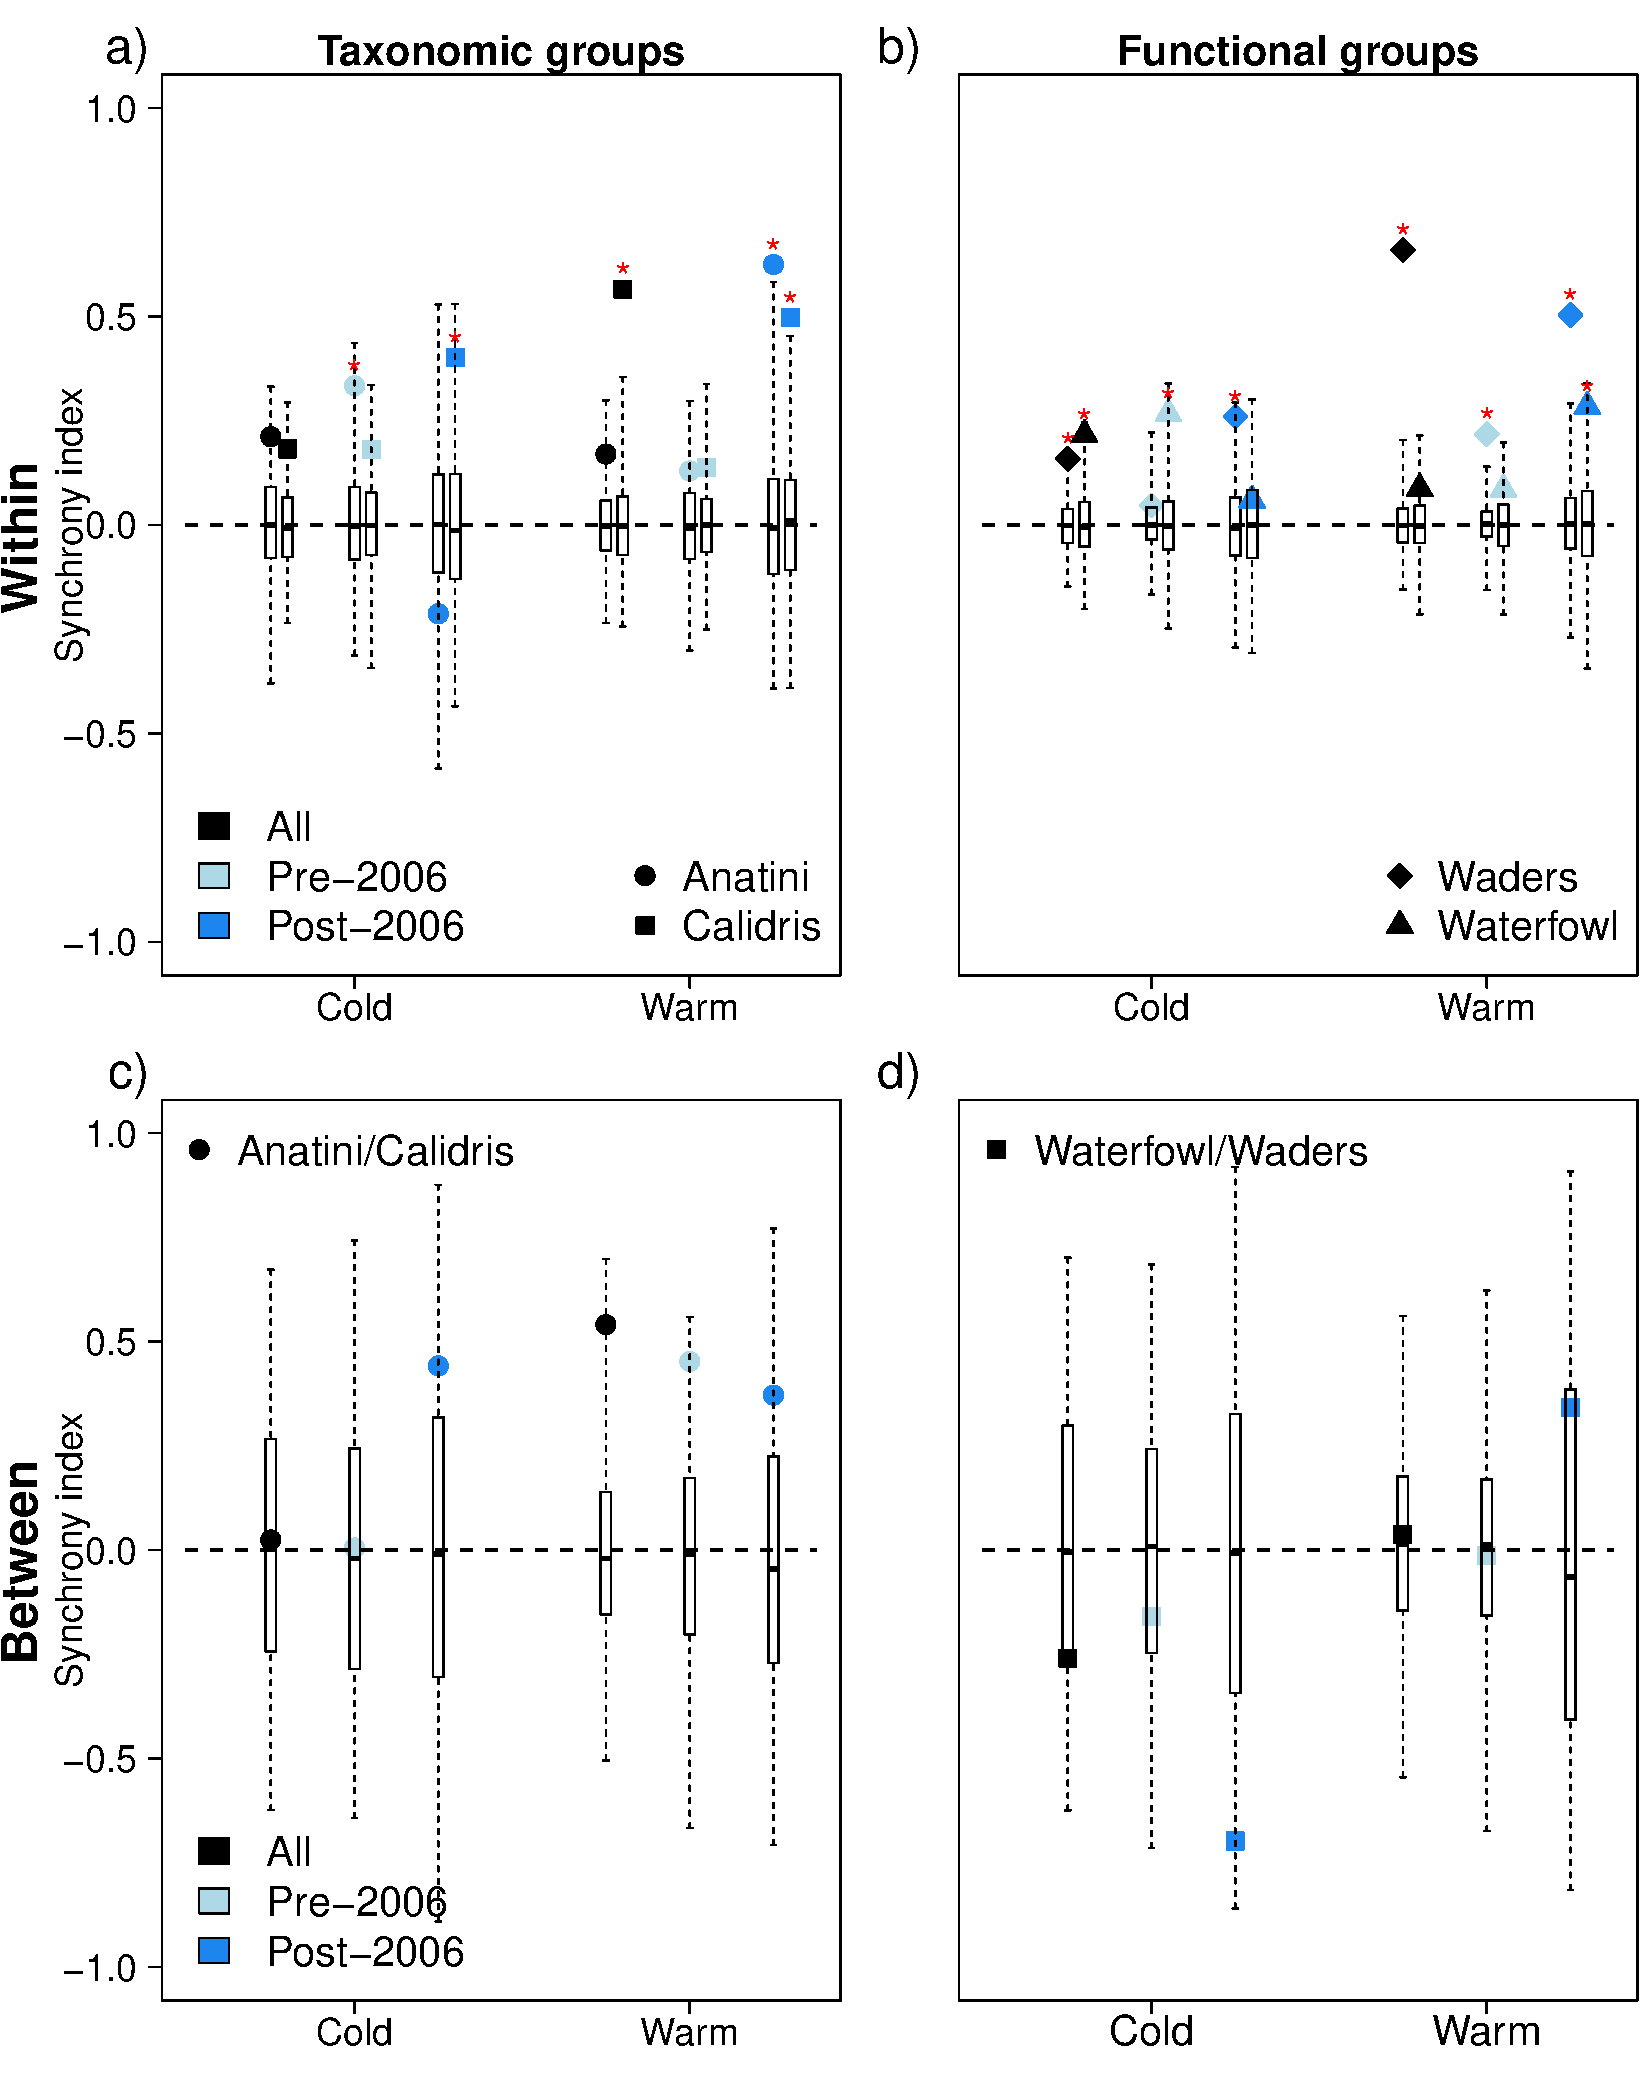
\includegraphics[width=0.85\textwidth]{Fig2_new3_JAE_abundances_NOTscaled}
\par\end{centering}
\caption{Gross' synchrony index ($\eta$) as a function of the season (cold
and warm seasons), calculated \emph{within} (top, a-b) and \emph{between}
(bottom, c-d) groups. The groups considered were different taxonomic
groups (\emph{Anatini}, \emph{Calidris}, left a-c) or functional groups
(waders vs waterfowl, right b-d). The index was computed in each panel
on the whole dataset (black) or using two periods: before and after
2006 (light and dark blue), the year of the change in water level
management. Boxplots indicate the distribution of $\eta$ under the
null hypothesis (independent species) and filled symbols correspond
to the observed values. Red stars correspond to synchrony values significantly
different from the null model, at the 10\% threshold with a Benjamini-Hochberg
correction. \label{fig:Gross-synchrony-index}}
\end{figure}

We thus find contrasted results regarding the effect of the management
change on synchrony within guilds or within the whole bird community,
depending on the type of analyses. Year-to-year analyses yield unclear
results for both guilds. At shorter (one or two months) and longer
(five years) timescales though, wavelet analyses show that the management
change may decrease synchrony and even promote compensation. 
\begin{figure}[H]
\begin{centering}
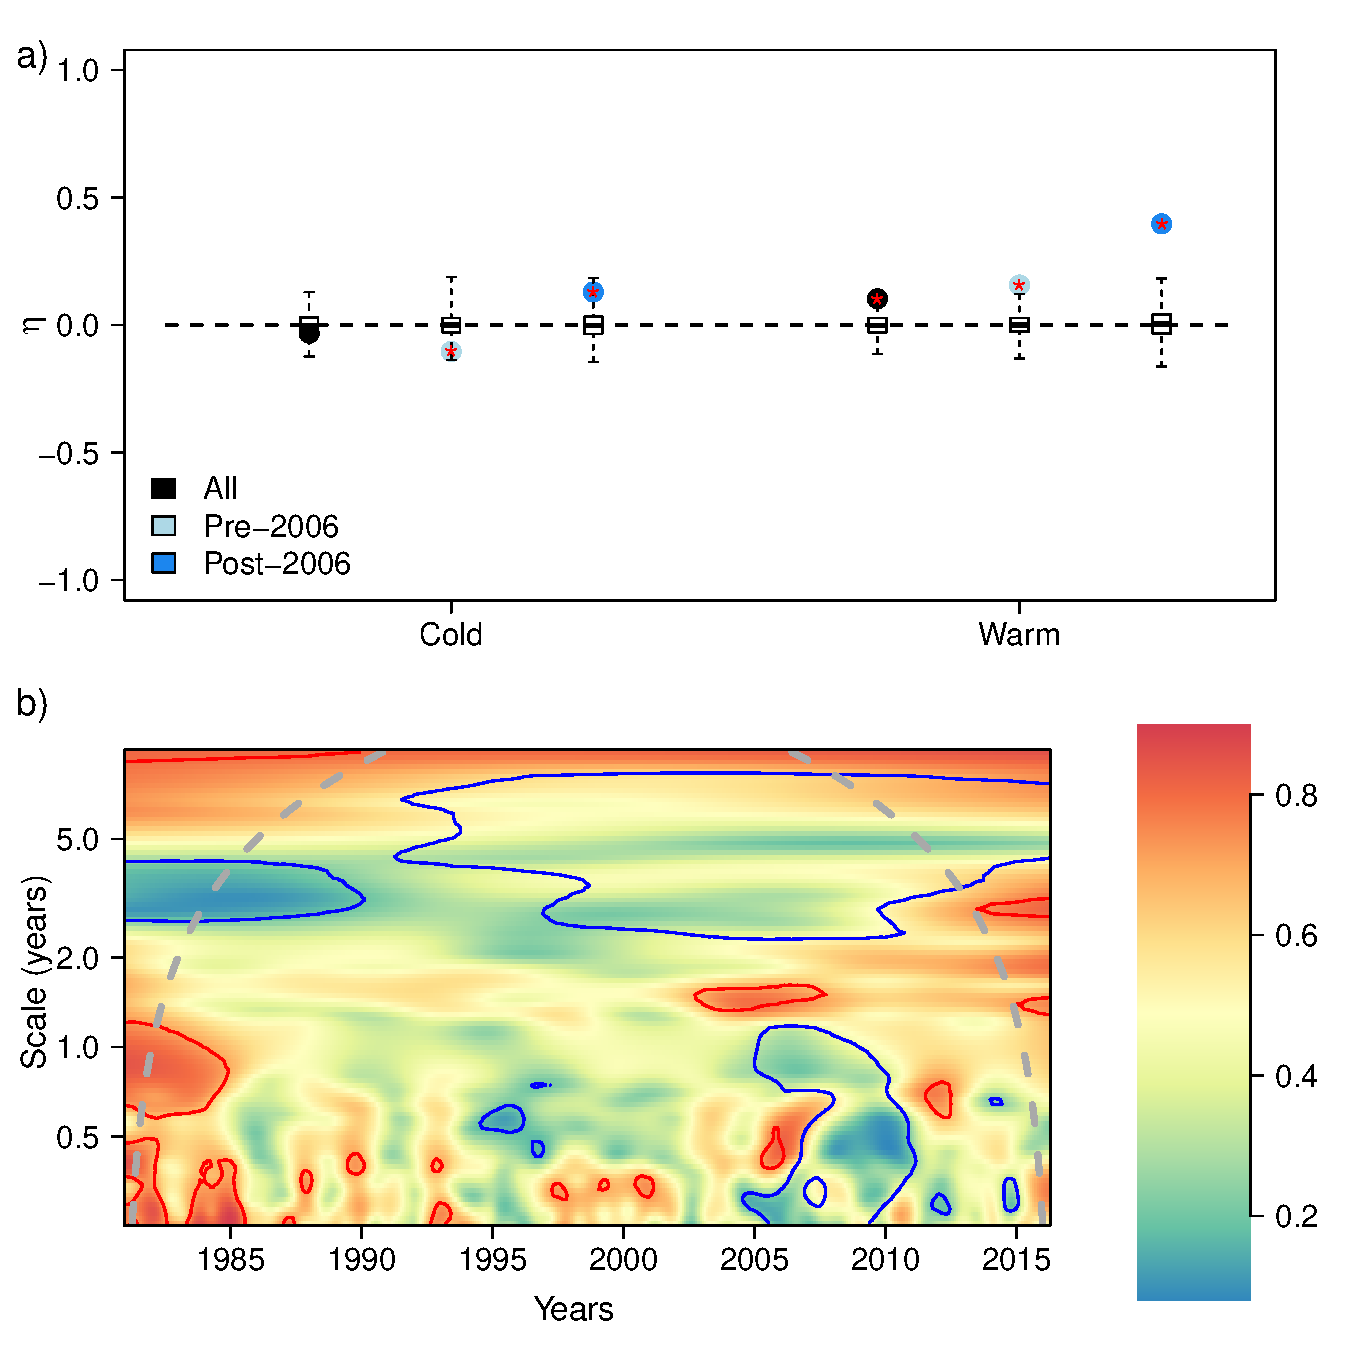
\includegraphics[width=0.95\textwidth]{synchrony_indices_frequent_abundances_NOTscaled_with1000rand_nocorrection_smallgrid_IAAFT_corrected_loc}
\par\end{centering}
\caption{Synchrony indices for the whole community of frequently observed birds.
Panel a) presents yearly synchrony ($\eta)$ for both seasons and
b) the wavelet modulus ratio ($\rho$). The latter index scales from
0 (compensation, blue color) to 1 (synchrony, red color). Red and
blue lines respectively delineate regions of significantly lower and
higher synchrony than the null model (independently fluctuating species,
but conserving their original Fourier spectrum), at the 10\% level.
\label{fig:synchrony-whole-comm}}
\end{figure}
\begin{figure}[H]
\begin{centering}
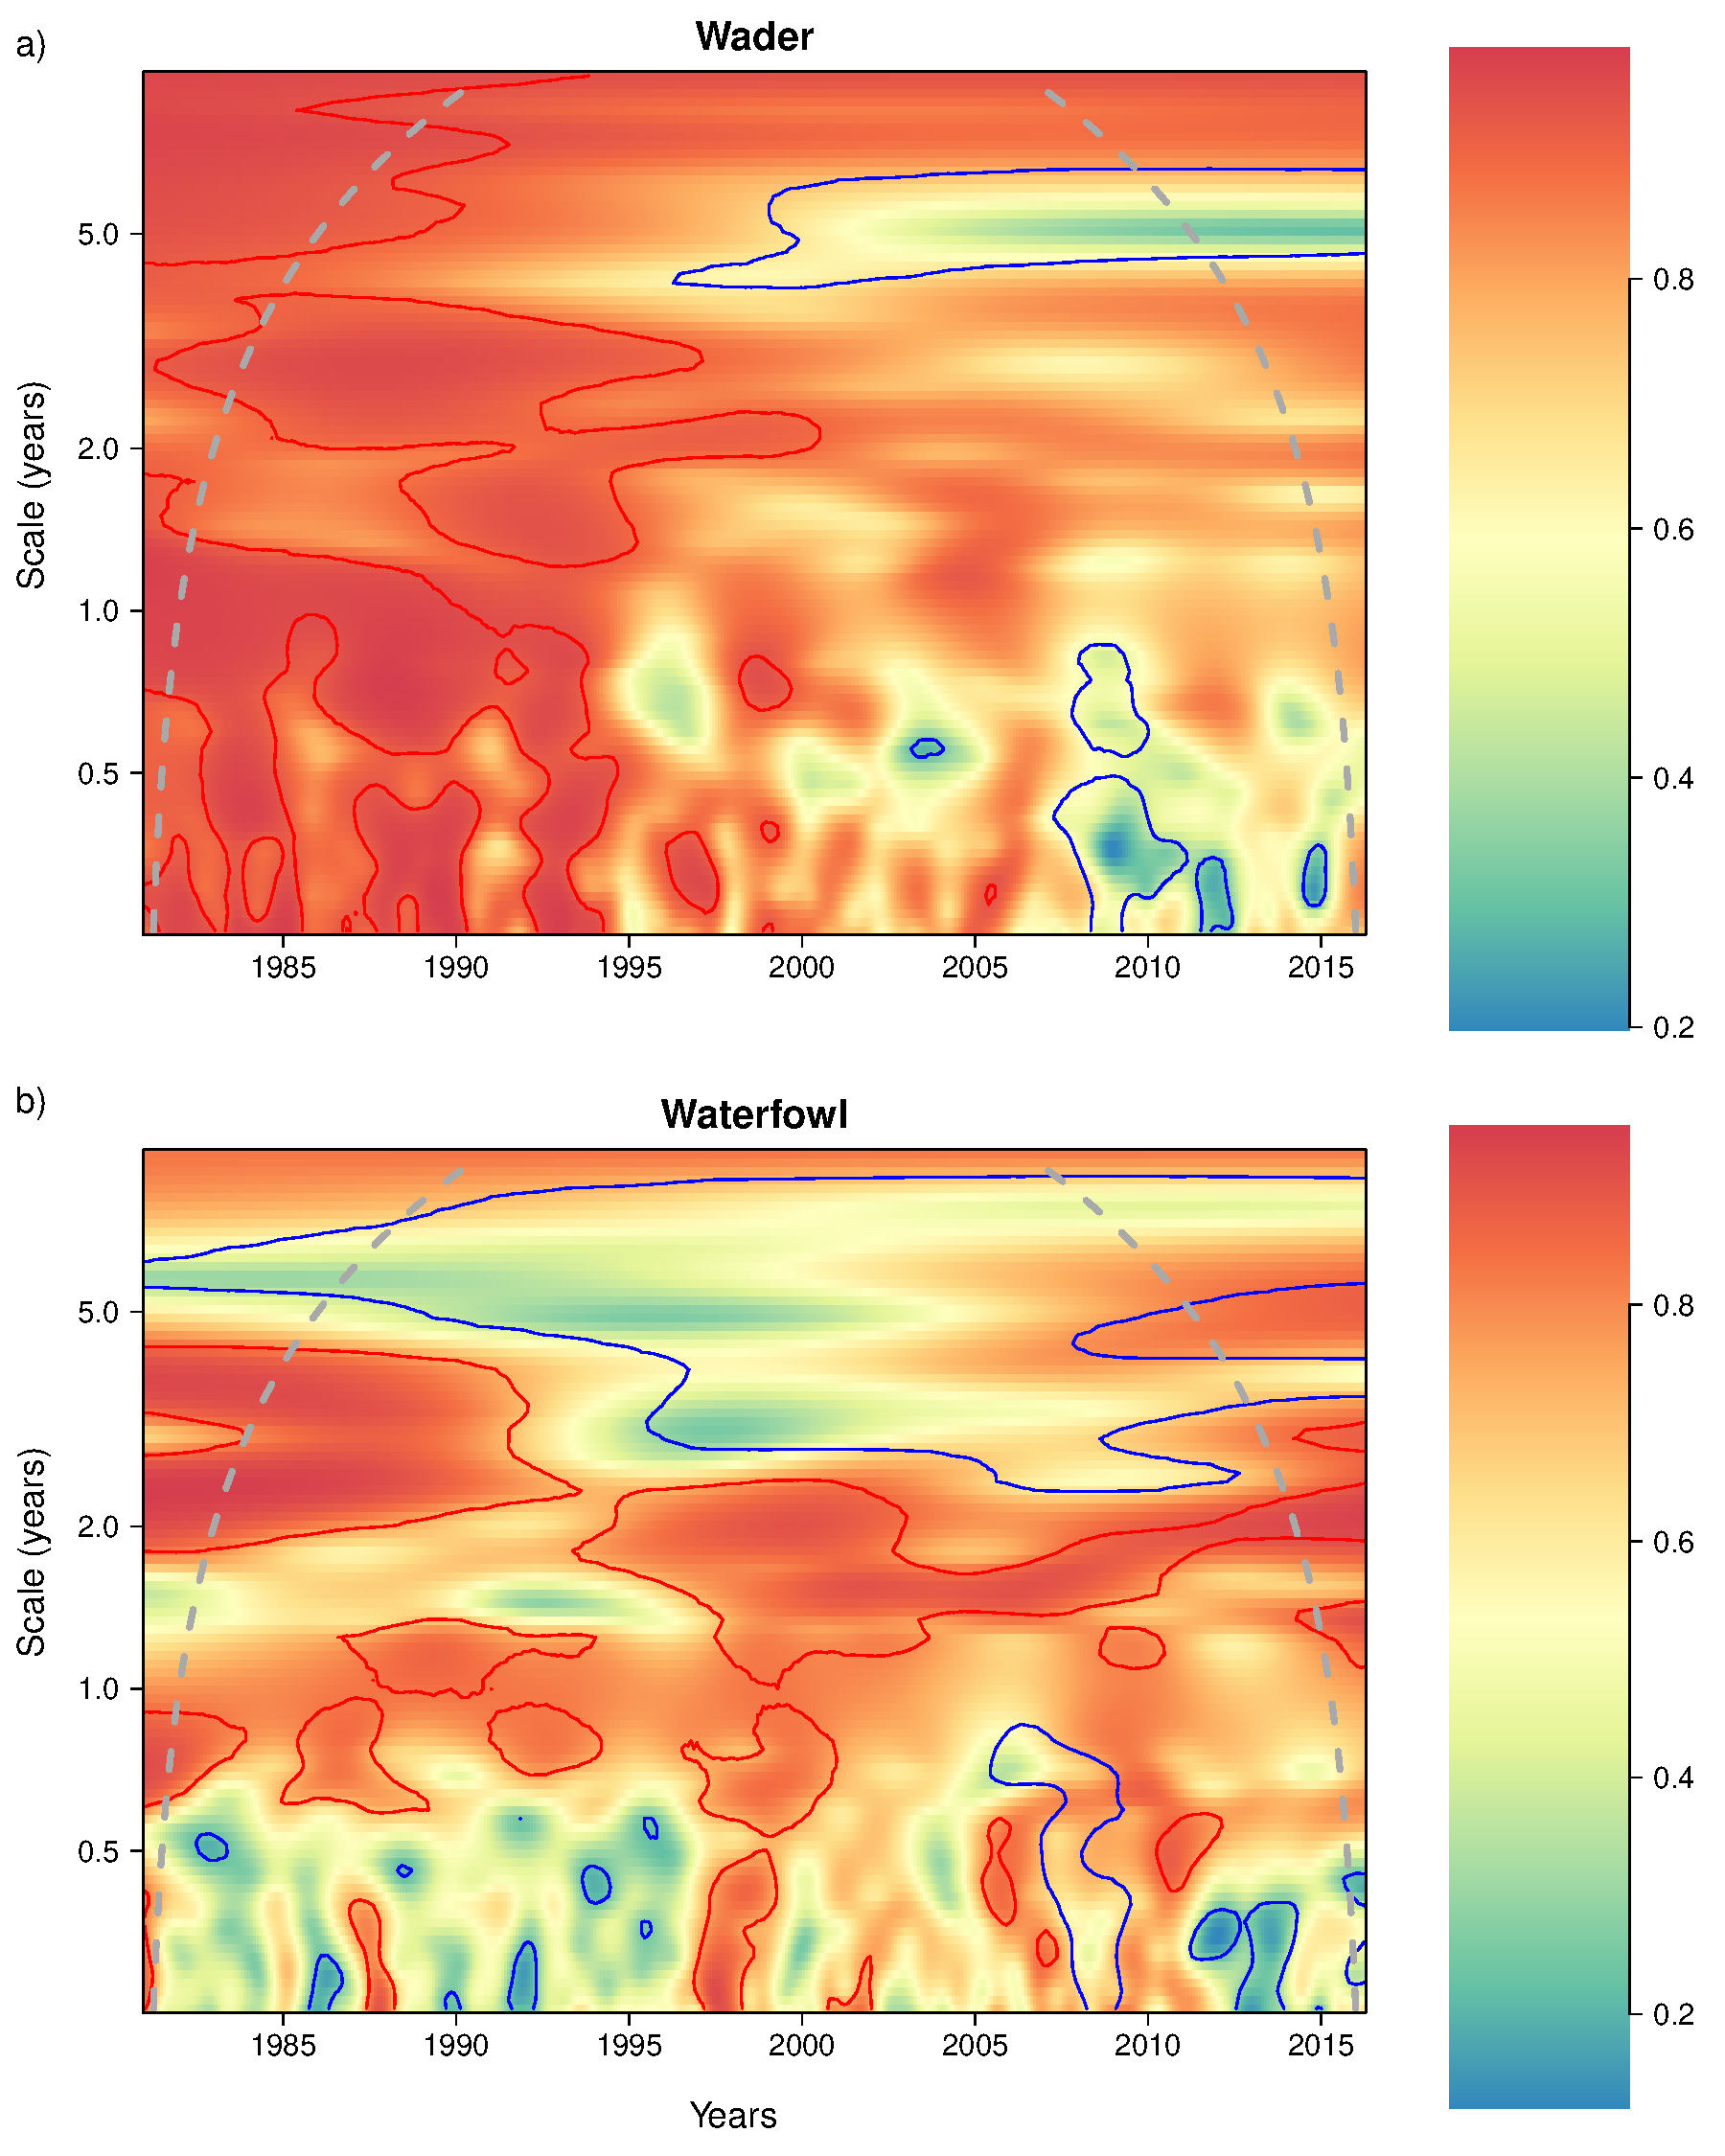
\includegraphics[width=0.95\textwidth]{wavelet_wader_waterfowlabundances_NOTscaled_with1000nocorrection_smallergrid_IAAFT}
\par\end{centering}
\caption{Wavelet modulus ratio ($\rho$) for a) the wader community and b)
the waterfowl community. The index $\rho$ scales from 0 (compensation,
blue color) to 1 (synchrony, red color). Red and blue lines respectively
delineate regions of significantly lower and higher synchrony than
the null model (independently fluctuating species, but conserving
their original Fourier spectrum), at the 10\% level. \label{fig:Wavelet-modulus-ratio}}
\end{figure}


\subsection*{Synchrony between phylogenetic or functional groups}

More easily interpretable results can be found when we examine synchrony
vs compensation between functional groups (Fig. \ref{fig:Gross-synchrony-index}d).
Since we consider only two functional or phylogenetic groups, the
\citet{gross2013species} index reduces to a simple correlation between
two groups. \emph{Anatini} and \emph{Calidris} are positively correlated
in the warm season (for all periods), and have unclear correlations
during the cold season (Fig. \ref{fig:Gross-synchrony-index}c). In
contrast, waders and waterfowl are negatively correlated during the
cold season and positively correlated during the warm season (Fig.
\ref{fig:Gross-synchrony-index}d). Although the negative correlation
is not statistically significant, it is consistent for both pre- and
post-2006 periods.

\subsection*{Synchrony in a small module with known competition}

Compensation could be expected upon visual inspection of the time
series of the two groups formed by cormorant on the one hand, and
little egret plus grey heron (summed as a small functional group)
on the other hand (Fig. \ref{fig:Time-series-of}, though see SI Appendix
S3 for alternative representations). However, we see on Fig. \ref{fig:Time-domain-(top)-and}
that synchrony is in fact the rule around the annual scale and below,
when considering the wavelet modulus ratio. We wondered if the patterns
in Fig. \ref{fig:Time-series-of} were caused by the use of a log
scale, but we found that in fact the correlation was higher rather
than lower on the log scale (Appendix S3). However, over long temporal
scales ($\sim$ 8 years) we observe consistent compensation, which
could correspond to the slow change in composition observed within
this small community module, that was already visible on the abundance
time series plot (Fig. \ref{fig:Time-series-of}). There is some statistically
significant compensation over shorter timescales as well, but only
at very specific times. The absence of marked compensation at short
temporal scales may be an inevitable consequence of the difference
in the amplitude of temporal variation between the two groups (Appendix
S8), as opposite annual phases for the two time series can be observed
before 2000 (Fig. \ref{fig:Time-series-of}).

\begin{figure}[H]
\begin{centering}
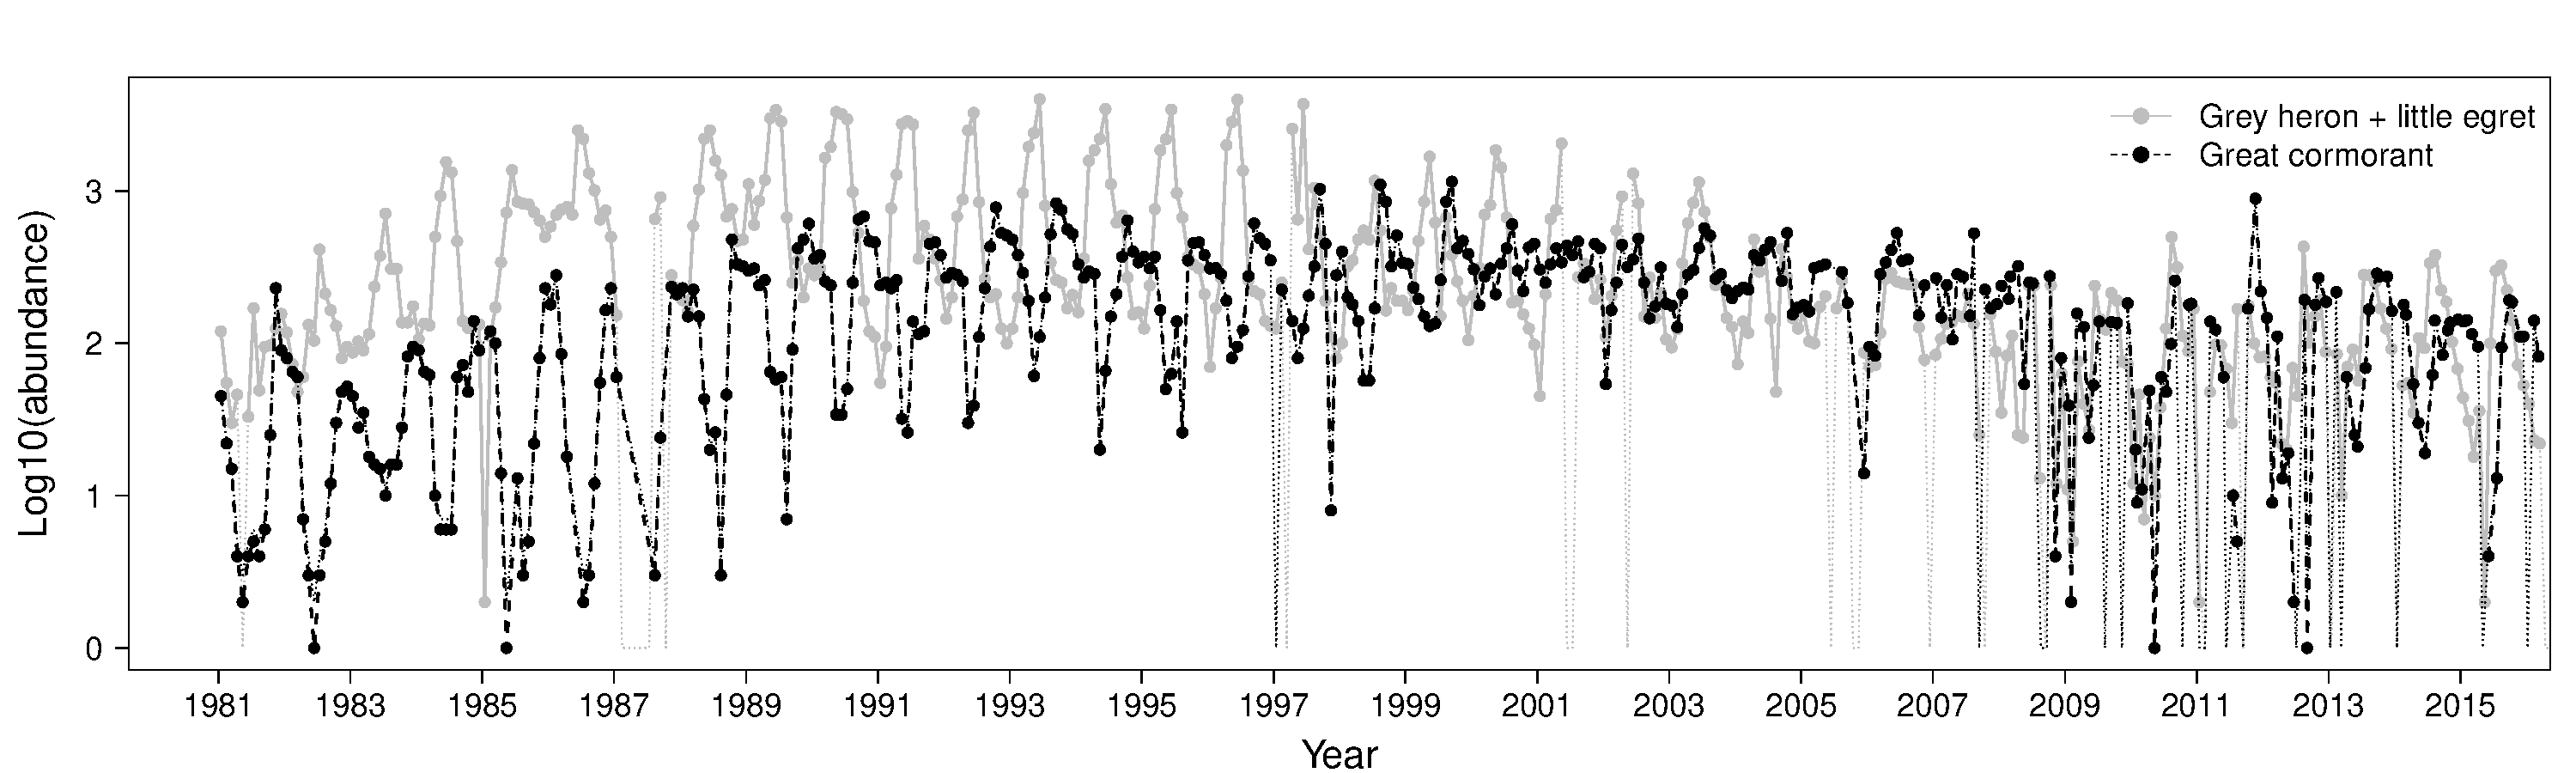
\includegraphics[width=1.1\textwidth]{abundance_3species}
\par\end{centering}
\caption{Time series of great cormorant abundance (dash-dotted black line),
as well as summed abundances of grey heron and little egret (solid
grey line). \label{fig:Time-series-of}}
\end{figure}

\begin{figure}[H]
\begin{centering}
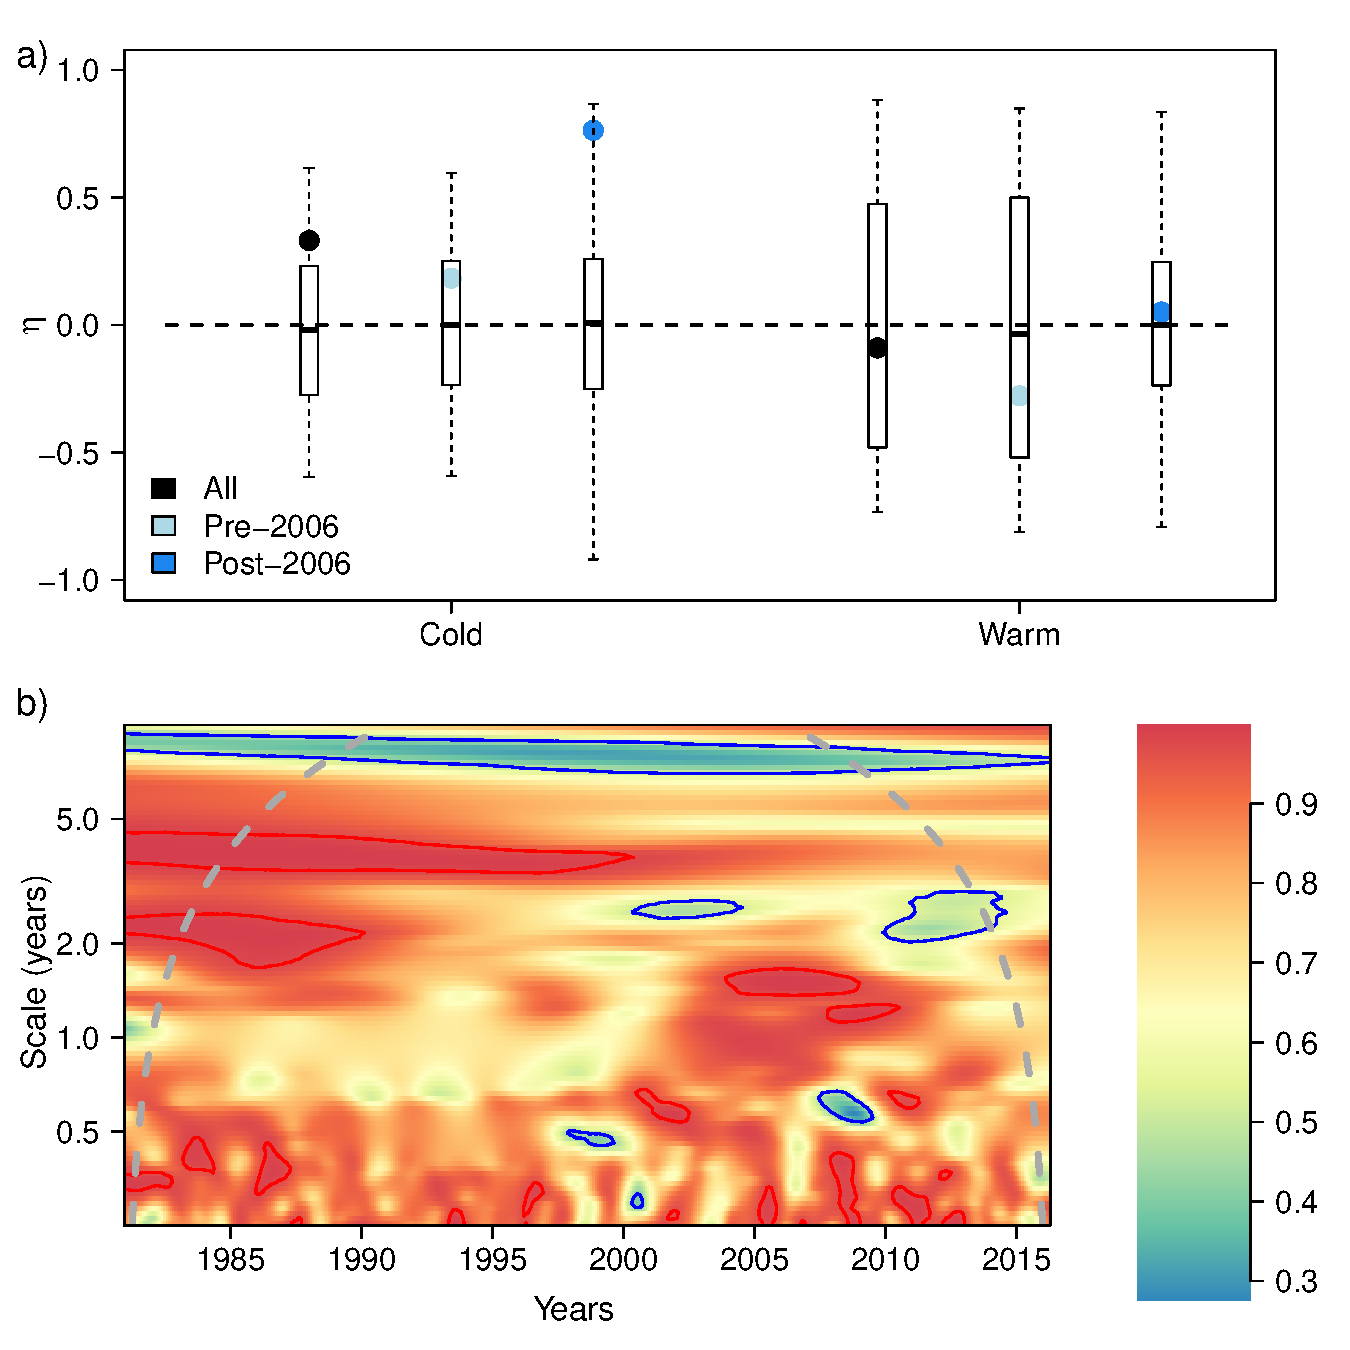
\includegraphics[width=0.99\textwidth]{triad_synchrony_2panels_abundances_NOTscaled_NOlog_test_with1000rand_nocorrection_smallgrid_IAAFT}
\par\end{centering}
\caption{Synchrony analyses of the group formed by cormorant vs egret and heron.
Panel a) presents yearly synchrony ($\eta)$ for both seasons and
b) the wavelet modulus ratio ($\rho$). The latter index scales from
0 (compensation, blue color) to 1 (synchrony, red color). Red and
blue lines respectively delineate regions of significantly lower and
higher synchrony than the null model (independently fluctuating species,
but conserving their original Fourier spectrum), at the 10\% level.
\label{fig:Time-domain-(top)-and}}
\end{figure}


\section*{Discussion}

Between-species compensation was not found across years (for two separate
seasons), synchrony between species being the rule. In other words,
there was no widespread ``functional compensation'' (\textit{sensu}
\citealt{gonzalez2009causes}) \emph{within} genera or guilds in year-to-year
analyses of cold and warm seasons. Yet, summing the abundances of
species within a guild and comparing these total abundances of contrasted
guilds, it was possible to find compensation across years, during
the cold season corresponding to wintering birds (although the null
hypothesis of no correlation could not be rejected); that is, there
was compensation \emph{between} guilds. These results are robust to
using biomass in place of abundance (SI Appendix S4). A zoom on a
module of three species with known competition also revealed clear
compensation at scales $\approx8$ years. We elaborate below on these
findings.

\subsection*{Synchrony \emph{within} or \emph{between} guilds}

Given that we compare the level of synchrony/compensation within guilds
(with many species) and between guilds (with only a handful of groups),
we checked in Appendix S5, using the dynamical model of \citet{gross2013species},
if changing the number of ``compartments'' ($n$) in the index $\eta$
could affect its value. It did not have marked effects, unless the
number of compartments is equal to 2, in which case significance is
hard to achieve and some compensatory dynamics can be missed with
weak environmental response. Additionally, we found -- still using
this dynamical model -- that if two guilds respond in opposite ways
to a shared environmental driver, the stronger the response of growth
rates to the driver, the lesser the compensation indicated by $\eta$
at the whole community level. An intuitive explanation of this modelling
result is that when there are two groups and many species within a
group, a stronger forcing homogeneizes the dynamics within a group
as much as it creates differences between groups. This might explain
the low levels of compensation that we found in our empirical dataset,
at the overall wetland bird community level (Fig. \ref{fig:synchrony-whole-comm}),
in spite of the clear presence of two guilds (waders and waterfowl)
reacting in opposite way to a shared driver (here, water levels).
Analyses at several taxonomic/functional scales are therefore warranted
to be conclusive about compensation, which mirrors what was suggested
by earlier plant studies \citep[e.g.,][]{bai2004ecosystem}. Future
case studies with more than two main functional groups may be instructive,
to challenge the generality of our findings.

We used correlation between the summed abundances of closely related
species (species within the \textit{Anatini }\textit{\emph{tribe}}
vs species within the \textit{Calidris} genus) or the summed abundances
of functionally similar species (waders vs waterfowl) to uncover compensation.
The functional group classification produced some compensation between
guilds while the taxonomic classification did not, despite the contrasted
habitat preferences of these two phylogenetic groups. Using functional
groups therefore produced more logical results, although as we stressed
above, the null hypothesis of no compensation at the yearly scale
could not be rejected, which may be due to the low power of the test
when comparing two groups.

We expected to see compensation at the ``functional group scale''
for both cold and warm seasons. The separation of seasons allowed
to differentiate summer residents (some of whom may be breeding) and
wintering birds, in order to remove the overwhelming influence of
the seasonal migratory cycle. In both of those seasons though, we
had reason to expect waders and waterfowl to have different environmental
preferences. Instead, waders and waterfowl were found to correlate
negatively only during the cold (wintering) season. A simple explanation
is that the reserve might be closer to its carrying capacity for these
species in winter, so that space is limited and increases in one functional
group are compensated by decreases in the other. The dominant species
in each guild (Fig. \ref{fig:Temporal-trends}), such as \emph{C.
alpina} for waders and \emph{A. crecca} for waterfowl, are migratory
species which are much more abundant in winter than summer in that
area, which adds to the plausibility of the reserve reaching carrying
capacity. Of course, the space constraint should not be taken too
literally: birds are obviously mobile and do forage outside of the
reserve (e.g., waders moving to the nearby Arcachon bay mudflats),
but there are costs to those movements (energetics, mortality risk
due to nearby hunting) which make the reserve a very attractive wintering
site where birds both rest and forage to some degree. Packing even
more birds over its 120 ha may just not be feasible, so that increases
in one guild result in decrease in the other. Compensation might
therefore be easier to detect during the cold season because the study
area is ``filled'', and it is not detected in our warm season (May
to August) because there are less birds overall.

It may be better to say that we detected ``compensation'' rather
than ``compensatory dynamics'' between bird species \citep{gonzalez2009causes},
if compensatory dynamics is thought to result from births and deaths,
i.e., population dynamics. Indeed, the observed long-term changes
in species composition (more waders, proportionally less waterfowl;
Appendix S2) is likely due to an increased inflow of birds preferring
low water levels (waders), and outflow of birds preferring high water
levels (waterfowl), under an overall space constraint (at least in
winter, as we explained above). Bird settlement decisions for both
winter and spring/summer seasons are the proximal causes of bird species
composition in the reserve, rather than population dynamics. However,
it would be incorrect to conclude that because the local compensation
in winter that we found results from bird behaviour, it is disconnected
from regional-scale community dynamics: which species are present
in the reserve - safe from hunting - affects ultimately their survival
and reproductive success, which then feeds back into the regional-scale
community dynamics. 

\subsection*{Effect of the change in management on synchrony}

Although we performed a first set of analyses using the whole time
series, we have also performed year-to-year analyses pre- and post-2006.
The reason for these additional analyses is that a marked change in
management occurred around 2006, after which the water levels were
lower. Separating pre-/post-2006 and comparing to the previous analyses
allows to disentangle the effect of the ``normal'' dynamics from
the effect of this management change. Pre- and post-2006 analyses
showed very little differences with whole time series analyses for
either the warm or cold season. However, in the wavelet modulus ratio
analyses, we see at monthly or 5-year timescales more compensation
after 2006 for waders; this could reflect that the community is becoming
saturated with waders. The effects of disturbances on the level of
synchrony or compensation are likely idiosyncratic: for instance,
\citet{keitt_coherent_2008} found increased synchrony after disturbance
while \citet{klink_functional_2019} found no clear effect.

\subsection*{Synchrony in a small module with known competition}

We now zoom in on the cormorant-heron-egret module, for which we knew
beforehand that competition for resting and roosting sites in the
summer season occurs between, on the one hand, great cormorants, and
on the other hand, little egrets and grey herons (C. Feign?, pers.
obs.). Abundance time series suggested some negative correlation,
but it was not found in year-to-year analyses for which synchrony
(or an absence of relation) dominates. Instead, we find that compensation
mostly occurs on a scale of 8 years, much above the annual scale,
which is a likely consequence of the slow shift in frequencies of
cormorants and little egrets / grey herons. The reason why we do not
find a compensation at the monthly to annual scale pre-2000 in spite
of some opposition of annual phases may be related to the large difference
in the amplitude of short-term temporal variation between the two
groups. When one functional group or species dominates the temporal
variation, as shown in SI Appendix S8, its dominance of temporal variation
can forbid the occurrence of compensation since by definition no increase
in the numbers of the species that fluctuate less may compensate for
the decreases in the species that fluctuate more (and vice versa).

\subsection*{Conclusion and perspectives for theory}

Overall, our results suggest to search for compensation more often\emph{
between} rather than \emph{within} functional groups, and over relatively
long timescales, above the typical temporal autocorrelation of the
dominant driver (e.g., above 5 years if the main driver is a seasonal
climate). This rejoins the recent findings of \citet{klink_functional_2019}
who found that increased functional differences between species tend
to decrease synchrony in beetles, as well as earlier results of \citet{bai2004ecosystem}
on negative covariation of plant functional groups. Our suggestion
goes against calls to search for compensation within closely related
species but at very short timescales \citep{vasseur2007spectral,gonzalez2009causes},
below the timescale of the main synchronizing seasonal environmental
driver, in order to filter out precisely its synchronizing effect.
Searching for compensation at temporal scales below the seasonal abiotic
driver (e.g., temperature) was partly motivated by studies on plankton
whose population dynamics are usually much faster than the dominant
abiotic driver, with short generation times, so that the effects of
competition may be manifest at the scale of a few weeks or months.

In theory, we could have expected compensation to manifest also at
the smallest temporal scale of our survey (monthly). Indeed, the community
dynamics in our case are driven by the movements and settlement decisions
of birds, reacting to perceived food and space availability, rather
than by births and deaths directly. Such behavioural dynamics can
certainly be much faster than bird population dynamics, and could
operate at the scale of weeks or months. However, such compensation
due to short-term movements was not observed except perhaps in some
years. We suspect that because many species share common abiotic drivers
(e.g., disturbances due to nearby hunting, local climatic conditions)
fluctuating even within a single season, their dynamics can be synchronized
by these drivers at monthly temporal scales. It is noteworthy that
even in planktonic systems, the temporal scale of compensation has
often been found to be well above that of the forcing driver \citep{keitt_coherent_2008,brown2016compensatory}.
Thus our findings reinforce previous suggestions to search for compensation
over relatively long timescales (several years for vertebrates or
plants).

The attractor of community dynamics, i.e., the shape of community
trajectories in phase space, seems to be more or less an annual cycle
here: the dominant species fluctuate seasonally, but even though there
are shifts in some species dynamics, no abundant species seem to exhibit
violent multi-year oscillations. If we had to describe our community
mathematically, a dynamical model with a stable fixed point forced
by seasonality and some noise would probably be appropriate. This
mild fluctuation scenario somehow contrasts with the dynamics of other
communities, such as insect pests, that have quite often multi-year
cycles (on top of seasonal cycles, for multivoltine species), with
possibly strong indirect interactions between similar species mediated
by predators and parasitoids \citep{murdoch2003consumer}. In the
latter context of internally-generated variability (``Endogenous
compensatory cycles\textquotedbl{} in \citealp{gonzalez2009causes}),
compensation may be more likely: \citet{klapwijk2018transient} recently
reported only transient synchrony between species of moths, that typically
exhibit such multi-year fluctuations.

In many ways, searching for abundance compensation using biodiversity
time series data is searching for needles in a haystack: only some
specific temporal and functional/taxonomic scales allow to see compensation
whilst numerous confounding factors make the community co-vary positively
at all other scales \citep{vasseur_synchronous_2014}. When a common
species fluctuates much more than the rest, this can also lessen or
forbid compensation. Thus, although the knowledge of specific biological
mechanisms increasing the densities of some species at the expense
of others can help, synchrony will likely dominate community-level
time series data for closely related species, even in species that
compete strongly \citep{ranta_detecting_2008,loreau_species_2008}.
This is true even in cases of known mechanisms of competition for
space or shifts in community composition due to abiotic changes affecting
differentially species preferences, as in this study. We therefore
suggest that ``zooming out'' functionally (considering summed abundances
of dissimilar functional groups) and temporally (considering temporal
scales well above the periodicity of the dominant abiotic driver)
may often be the best strategy to see the compensation that will inevitably
manifest at some scales, if the community-level biomass is to be maintained
within bounds in the long run.

\subsection*{Acknowledgements}

We warmly thank the birdwatchers and staff of the Teich Reserve/Landes
Gascogne regional park who contributed to data collection over the
years, as well as LPO Aquitaine for helping us retrieve the raw data.
Constructive feedback by six referees -- Roel van Klink, Mike Fowler,
and four anonymous others -- as well as three associate editors considerably
improved the manuscript. The data collection was supported by the
Landes Gascogne regional park as well as the Teich municipality, while
data analysis was funded by LabEx COTE (ANR-10-LABX-45).

\subsection*{Data accessibility}

All the code and data used for analyses are available at \url{https://github.com/fbarraquand/BirdTimeSeries_Teich}
and archived at Zenodo {[}will be done for the final version{]}, DOI:XX-XXX
(Picoche, Aluome \& Barraquand, 2020).

\subsection*{Authors' contributions}

FB, LC and CF designed the original project. CF coordinated the data
collection and provided knowledge on functional groups. CA, FB and
CP standardized the bird abundance database and performed exploratory
analyses. Final statistical analyses were designed by FB and CP, and
coded mostly by CP. FB and CP led the article writing, with inputs
from all authors.

}\end{linenumbers}

\bibliographystyle{besjournals}
\bibliography{BiblioTeich}

\end{document}
